\documentclass[../../main.tex]{subfiles}

\graphicspath{{../../image/}{../../figure/}}

\begin{document}

\section{可视化训练好的 CNN}\label{section:ch10-可视化训练好的CNN}

本节介绍探索现代深度 CNN 所学习到的特征，你将看到它们与哺乳动物视觉皮层性质的一些显著相似之处。

\subsection{视觉皮层}\label{subsection:ch10-视觉皮层}

研发 CNN 的大部分动机来自神经科学的开创性研究，这些研究深入了解了包括人类在内的哺乳动物视觉处理的本质。来自视网膜的电信号通过位于大脑后部的视觉皮层中的一系列处理层进行转换，其中神经元组织成二维片，每个二维片形成二维视野的映射。在这些开创性研究中，Hubel and Wiesel (1959) 测量了当向猫的眼睛呈现视觉刺激时，猫的视觉皮层中单个神经元的电响应。他们发现，一些称为“简单细胞”的神经元对视觉输入有强烈的响应，这些视觉输入朝向特定角度的简单边缘，位于视野内的特定位置。而其他刺激在这些神经元中产生的响应相对较少。更详细的研究表明，这些简单细胞的响应可以使用 Gabor 滤波器来建模，Gabor 滤波器是由下式定义的二维函数：
\begin{align}
  G(x,y) = A\exp\left(-\alpha\tilde{x}^2-\beta\tilde{y}^2\right)\sin\left(\omega\tilde{x}+\phi\right),
  \label{align:ch10-Gabor滤波器}
\end{align}
其中
\begin{align}
  \tilde{x} = (x-x_0)\cos(\theta)+(y-y_0)\sin(\theta),
  \label{align:ch10-Gabor坐标旋转1}
\end{align}
\begin{align}
  \tilde{y} = -(x-x_0)\sin(\theta)+(y-y_0)\cos(\theta).
  \label{align:ch10-Gabor坐标旋转2}
\end{align}
\eqref{align:ch10-Gabor坐标旋转1}和\eqref{align:ch10-Gabor坐标旋转2}表示坐标系旋转角度 $\theta$，因此\eqref{align:ch10-Gabor滤波器}中的 $\sin(\cdot)$ 项表示朝向极角 $\theta$ 方向的正弦空间振荡，频率为 $\omega$，相位角为 $\phi$。\eqref{align:ch10-Gabor滤波器}中的指数因子旨在创建一个衰减包络，将滤波器置于点 $(x_0,y_0)$ 的邻域内，衰减速率由 $\alpha$ 和 $\beta$ 控制。\eqref{align:ch10-Gabor滤波器}定义的 Gabor 滤波器示例如\cref{figure:ch10-Gabor滤波器}所示。

\begin{definition}[Gabor 滤波器]\label{definition:ch10-Gabor滤波器}
称由\eqref{align:ch10-Gabor滤波器}--\eqref{align:ch10-Gabor坐标旋转2}定义的二元函数 $G:\mathbb{R}^2\to\mathbb{R}$ 为 \textbf{Gabor 滤波器}，其中 $A>0$ 为振幅，$\alpha,\beta>0$ 为包络在 $\tilde{x},\tilde{y}$ 方向上的衰减速率，$\omega>0$ 为空间频率，$\phi$ 为相位角，$\theta$ 为朝向角，$(x_0,y_0)$ 为滤波器的中心位置，$(\tilde{x},\tilde{y})$ 是绕 $(x_0,y_0)$ 旋转 $\theta$ 后的局部坐标。
\end{definition}

% SUPPLEMENT: parent=definition:ch10-Gabor滤波器; kind=motivation; location=紧随其后的 remark（重构新增）
\begin{remark}（重构新增）
Gabor 滤波器是“Gauss包络乘正弦条纹”，这个形式的两部分各自对应一个可验证的性质。正弦因子 $\sin(\omega\tilde{x}+\phi)$ 沿 $\tilde{x}$ 方向振荡、沿 $\tilde{y}$ 方向不变，因此它是一个方向选择性滤波器：只有与朝向 $\theta$ 垂直的边缘才会产生强响应，这正是简单细胞的朝向选择性。Gauss因子 $\exp(-\alpha\tilde{x}^2-\beta\tilde{y}^2)$ 使响应局限在 $(x_0,y_0)$ 附近，因此它是位置选择性的；$\alpha\neq\beta$ 时包络是椭圆的，允许滤波器在振荡方向上延伸更长（更窄的频带）。参数条件 $\alpha,\beta>0$ 不可省，否则包络发散、函数不再可积；$\omega>0$ 只是约定振荡的“正方向”，改变 $\omega$ 的符号等价于把 $\phi$ 平移 $\pi$。\eqref{align:ch10-Gabor坐标旋转2}中的负号保证 $(\tilde{x},\tilde{y})$ 是右手正交坐标，若写成正号则旋转方向相反，滤波器的朝向会与 $\theta$ 差一个镜像。
\end{remark}

\begin{figure}[htbp]
  \centering
  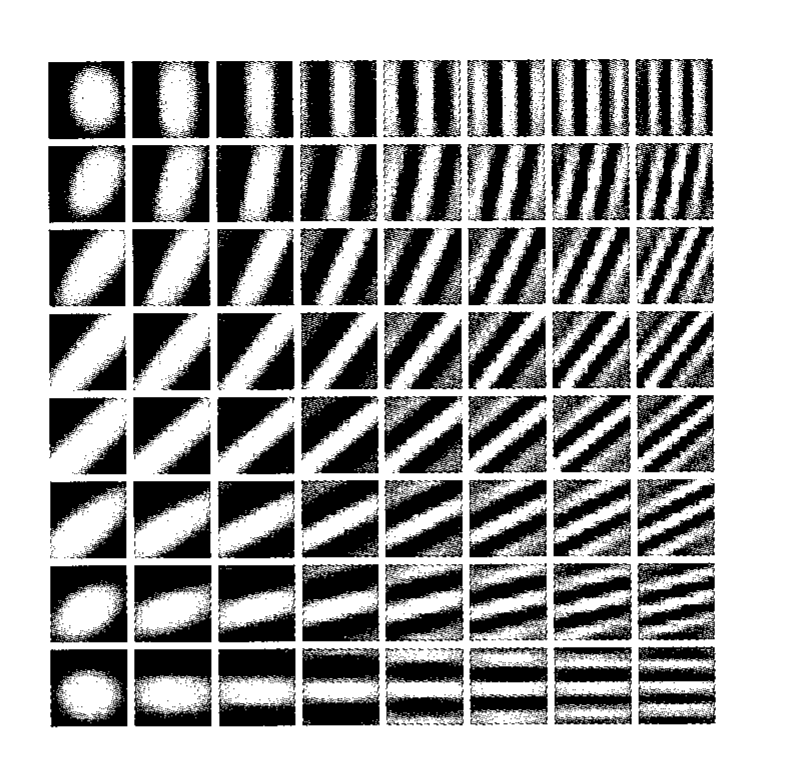
\includegraphics[width=0.42\textwidth]{ch10-fig10-11-gabor.png}
  \caption{\eqref{align:ch10-Gabor滤波器}定义的 Gabor 滤波器示例。朝向角 $\theta$ 从顶行的 $0$ 向底行的 $\pi/2$ 变化，频率从左列的 $\omega=1$ 向右列的 $\omega=10$ 变化。}
  \label{figure:ch10-Gabor滤波器}
\end{figure}

Hubel 和 Wiesel 还发现了“复杂细胞”的存在，这些细胞会响应更复杂的刺激，并且该刺激似乎是通过组合和处理简单细胞的输出得到的。这些响应对输入中的微小变化（例如位置偏移）表现出一定程度的不变性，类似于深度卷积网络中的池化单元。哺乳动物视觉处理系统的更深层对视觉输入的变换具有更具体的响应和更大的不变性。这种细胞称为“祖母细胞”，因为不论场景的位置、大小、照明或其他变换如何，当且仅当视觉输入与某些特定的概念（如祖母的头像）相对应时，这种细胞才能在理论上做出响应。这项工作直接启发了一种称为新认知机（neocognitron）（Fukushima, 1980）的深度神经网络的早期形式，它是卷积神经网络的先驱。新认知机支持多层处理，包括了具有共享权重的局部感受野和紧接着的局部平均或最大池化，以确保位置不变性。然而，新认知机缺乏端到端的训练过程，而依赖于无监督聚类算法进行贪婪的逐层学习。

\begin{definition}[新认知机]\label{definition:ch10-新认知机}
称满足下列条件的多层网络为\textbf{新认知机}（neocognitron）：每一层由若干二维单元片组成，每个单元只连接前一层的一个局部感受野，同一片内的单元共享权重；每个卷积型的层之后紧跟一个局部平均或局部最大池化层，以获得位置不变性；各层以无监督聚类算法逐层贪婪训练，而非端到端地最小化统一损失。
\end{definition}

% SUPPLEMENT: parent=definition:ch10-新认知机; kind=motivation; location=紧随其后的 remark（重构新增）
\begin{remark}（重构新增）
新认知机在结构上已经具备现代 CNN 的三要素：局部感受野、权重共享、池化；它缺少的是训练方式——贪婪逐层聚类无法把“分类错误”这一全局目标反传到前面的层，因此每一层学到的表示只能局部最优。定义把“逐层贪婪训练”写进对象本身，是为了说明它与 CNN 的差别不在前向结构而在学习规则。这也解释了为什么在反向传播（\cref{chapter:ch08-反向传播}）与大规模数据都具备之后，同样的结构才真正发挥作用。把池化紧接在卷积之后这一安排，正是后文\cref{subsection:ch10-池化}所沿用的模式。
\end{remark}

\subsection{可视化训练好的滤波器}\label{subsection:ch10-可视化训练好的滤波器}

假设我们有一个训练好的深度 CNN，我们希望了解隐藏单元学会了检测什么。对于第一个卷积层中的滤波器，这是相对直接的，因为它们对应于原始输入图像空间中的小块，我们可以将这些滤波器的网络权重直接可视化为小的图像块。第一个卷积层计算滤波器和相应图像块的内积，当内积较大时，隐藏单元将具有较大的激活。

\cref{figure:ch10-AlexNet滤波器}展示了一些在 ImageNet 数据集上训练好的 CNN 第一层滤波器示例。我们看到这些滤波器与\cref{figure:ch10-Gabor滤波器}中的 Gabor 滤波器之间存在显著的相似性。然而，这并不意味着卷积神经网络是大脑工作的良好模型，因为我们可以从各种统计方法中获得非常相似的结果（Hyv\"arinen, Hurri, and Hoyer, 2009）。这些特征滤波器表示的是统计自然图像的一般性质，它们对于自然和人工系统中的图像理解都被证明是有用的。

\begin{figure}[htbp]
  \centering
  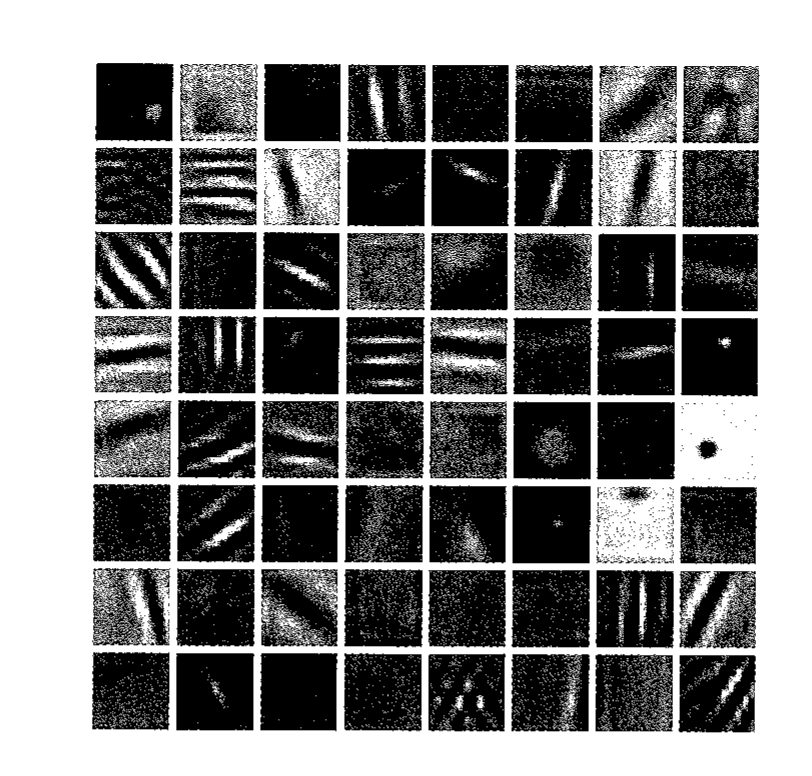
\includegraphics[width=0.45\textwidth]{ch10-fig10-12-alexnet滤波.png}
  \caption{AlexNet 第一层学习到的滤波器示例。注意，许多学习到的滤波器与\cref{figure:ch10-Gabor滤波器}中的 Gabor 滤波器具有惊人的相似性，它们对应于哺乳动物视觉皮层中活跃神经元检测到的特征。}
  \label{figure:ch10-AlexNet滤波器}
\end{figure}

虽然我们可以直接可视化第一层中的滤波器，但网络中的后续层更难解释，因为它们的输入不是图像小块，而是滤波器响应。一种方法（类似于 Hubel 和 Wiesel 使用的方法）是向网络提供大量图像小块，并观察哪些图像小块在任何特定隐藏单元中产生最大的激活值。\cref{figure:ch10-最强激活小块}显示了在网络的隐藏单元中产生最强激活的图像小块示例。该网络有 5 个卷积层，紧接着是两个全连接层，在包含 1 000 个类别的 130 万幅 ImageNet 图像上完成训练。我们看到一个自然的分层结构，第 1 层对边缘响应，第 2 层对纹理和简单形状响应，第 3 层显示对象的组成部分（如轮子），第 5 层显示整个对象。

\begin{figure}[htbp]
  \centering
  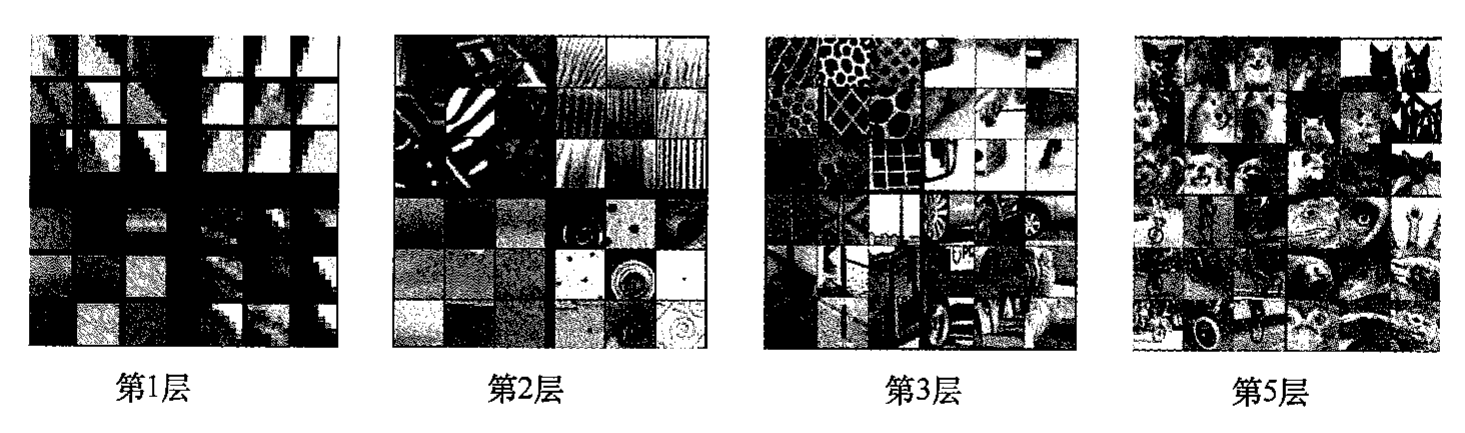
\includegraphics[width=0.9\textwidth]{ch10-fig10-13-最强激活小块.png}
  \caption{在网络的隐藏单元中产生最强激活的图像小块示例（取自验证集）。该网络有 5 个卷积层，在 ImageNet 图像上完成训练。针对 4 个随机选择的通道，每个对应层的特征图中的前 9 个激活排成了一个 $3\times 3$ 的网格。我们看到复杂性会随着深度的增加稳步增长——从第 1 层的简单边缘到第 5 层的完整对象［经 Zeiler and Fergus (2013) 授权使用］。}
  \label{figure:ch10-最强激活小块}
\end{figure}

我们可以扩展这种技术，使其不仅仅从验证集中选择图像小块，而且对输入变量进行数值优化，以最大限度地激活特定单元（Zeiler and Fergus, 2013; Simonyan, Vedaldi, and Zisserman, 2013; Yosinski et al., 2015）。如果我们选择某单元作为输出之一，则可以寻找最能代表相应类标签的图像。由于输出单元通常具有 softmax 激活函数，因此最好最大化输入 softmax 激活函数的预激活值，而不是直接最大化类概率，因为这样可以确保优化仅依赖于一个类。例如，假设我们想要寻找对类别“狗”产生最强烈响应的图像，那么如果我们优化 softmax 输出，由于 softmax 激活函数中的分母的存在，可能会使图像变得不那么像猫。然而，输出单元激活的无约束优化会导致单个像素值趋于无穷大，并且还会产生难以解释的高频结构，因此需要某种形式的正则化来找到更接近自然图像的解。Yosinski et al. (2015) 使用了一种正则化函数，该函数涉及像素值的平方和以及一个变换过程。该过程将基于梯度的更新替换为删除高频结构的模糊操作，并引入剪裁操作来将那些对类标签贡献很小的像素值设置为零，示例结果如\cref{figure:ch10-类最大化图像}所示。这种方法与对抗训练有关（参见\cref{chapter:ch17-生成对抗网络}）。

\begin{figure}[htbp]
  \centering
  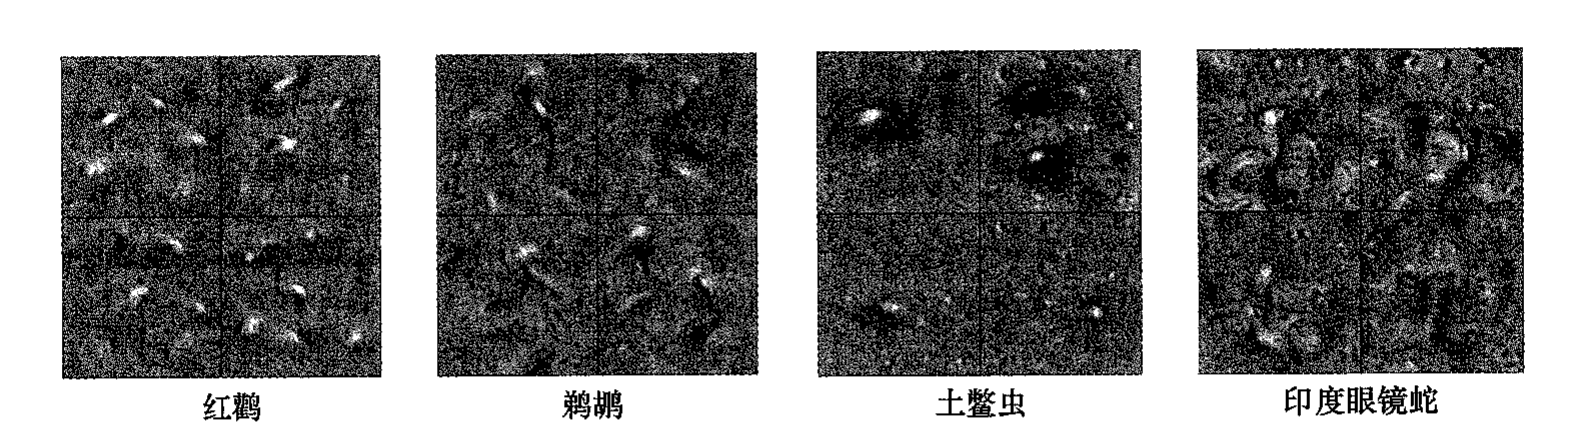
\includegraphics[width=0.88\textwidth]{ch10-fig10-14-类最大化图像.png}
  \caption{通过训练好的卷积分类器，对图像像素通道值最大化类概率生成的合成图像示例。图中显示了对于每一对象类别，通过不同正则化参数设置得到的 4 个不同的解［经 Yosinski et al. (2015) 授权使用］。}
  \label{figure:ch10-类最大化图像}
\end{figure}

\subsection{显著性图}\label{subsection:ch10-显著性图}

深入了解卷积网络所用特征的另一种方法是使用显著性图（saliency map），目的是在确定类标签时识别图像中最重要的区域。这最好通过研究最终卷积层来完成，因为该卷积层仍然保留了空间定位信息，该信息在随后的全连接层中会丢失，但它们具有最高级别的语义表示。对于给定的输入图像，Grad-CAM（Gradient Class Activation Mapping，梯度类激活图）方法（Selvaraju et al., 2016）首先在 softmax 输出之前，计算对于给定类别 $c$ 的输出单元预激活 $a^{(c)}$ 关于最终卷积层通道 $k$ 中所有单元预激活 $a_{ij}^{(k)}$ 的导数。对于该层中的每个通道，这些导数的平均值形式如下：
\begin{align}
  \alpha_k = \frac{1}{M_k}\sum_{i}\sum_{j}\frac{\partial a^{(c)}}{\partial a_{ij}^{(k)}},
  \label{align:ch10-GradCAM通道权重}
\end{align}
其中 $i$ 和 $j$ 用于索引通道 $k$ 的行和列，$M_k$ 是通道 $k$ 中的单元总数。然后，这些平均值被用于形成以下形式的加权和：
\begin{align}
  L = \sum_{k}\alpha_k A^{(k)},
  \label{align:ch10-GradCAM}
\end{align}
其中 $A^{(k)}$ 是包含元素 $a_{ij}^{(k)}$ 的矩阵。生成的数组与最终卷积层具有相同的维度，例如\cref{figure:ch10-VGG16架构}所示的 VGG-16 模型的维度为 $14\times 14$，并且可以用“热力图”的形式叠加在原始图像上，如\cref{figure:ch10-显著性图}所示。

\begin{definition}[显著性图与 Grad-CAM]\label{definition:ch10-显著性图}
设 $a^{(c)}$ 为类别 $c$ 在 softmax 之前的预激活，$a_{ij}^{(k)}$ 为最后一个卷积层第 $k$ 个通道在位置 $(i,j)$ 处的预激活。称按\eqref{align:ch10-GradCAM通道权重}算出的 $\alpha_k$ 为通道 $k$ 对类别 $c$ 的\textbf{权重}，称按\eqref{align:ch10-GradCAM}算出的矩阵 $L$ 为类别 $c$ 的 \textbf{Grad-CAM 显著性图}（saliency map）。
\end{definition}

% SUPPLEMENT: parent=definition:ch10-显著性图; kind=motivation; location=紧随其后的 remark（重构新增）
\begin{remark}（重构新增）
显著性图的定义把“哪些像素重要”转化为“哪些通道重要、以及这些通道在哪里激活”。\eqref{align:ch10-GradCAM通道权重}对空间位置取平均，是为了让权重与位置无关（否则热力图会退化成一堆逐点导数）；\eqref{align:ch10-GradCAM}再用该权重把各通道的激活图加权求和，于是 $L$ 与最后一个卷积层同尺寸。定义中要求 $a^{(c)}$ 是 softmax 之前的预激活而不是概率，因为概率经 softmax 归一化后所有类别的梯度相互耦合，单看某一类的概率导数会混入其他类的信息。注意 $L$ 可以取负值：负值表示该位置对类别 $c$ 起反作用，实际可视化时常截断为 $\max(L,0)$ 再归一化，这只是显示上的处理，不改变定义。
\end{remark}

\begin{figure}[htbp]
  \centering
  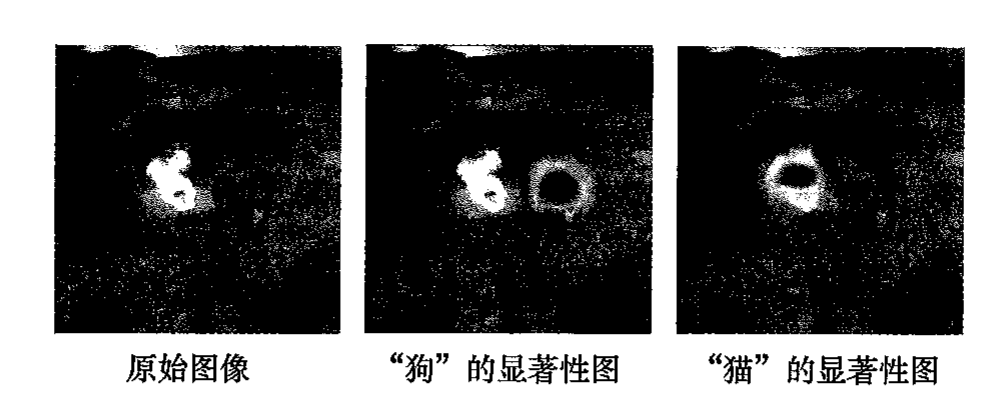
\includegraphics[width=0.6\textwidth]{ch10-fig10-15-显著性图.png}
  \caption{VGG-16 模型关于类别“狗”和“猫”的显著性图［经 Selvaraju et al. (2016) 授权使用］。}
  \label{figure:ch10-显著性图}
\end{figure}

\subsection{对抗攻击}\label{subsection:ch10-对抗攻击}

与输入图像像素值变化相关的梯度也可用于创建针对卷积网络的对抗攻击（adversarial attack）（Szegedy et al., 2013）。这类攻击以人类无法察觉的水平对图像进行非常小的修改，从而导致神经网络对图像分类错误。创建对抗性图像的一种简单方法是快速梯度符号（fast gradient sign）法（Goodfellow, Shlens, and Szegedy, 2014）。这涉及将图像 $\mathbf{x}$ 中的每个像素值更改为固定量 $\varepsilon$，符号由误差函数 $E(\mathbf{x},t)$ 相对于像素值的梯度确定。我们将得到一幅由下式定义的修改后的图像：
\begin{align}
  \tilde{\mathbf{x}} = \mathbf{x}+\varepsilon\,\mathrm{sign}\left(\nabla_{\mathbf{x}}E(\mathbf{x},t)\right),
  \label{align:ch10-快速梯度符号}
\end{align}
这里的 $t$ 是 $\mathbf{x}$ 的真实标签，误差 $E(\mathbf{x},t)$ 举例来说可以是 $\mathbf{x}$ 的负对数似然。使用反向传播可以有效地计算所需梯度（参见\cref{chapter:ch08-反向传播}）。在神经网络的常规训练中，可以通过调整网络参数来最小化误差，而\eqref{align:ch10-快速梯度符号}定义的修改会改变图像（同时保持训练好的网络参数固定），从而导致误差增加。通过保持 $\varepsilon$ 为较小的值，可以确保人眼无法察觉图像的变化。值得注意的是，这可以使网络以较高的置信度将图像分类错误，如\cref{figure:ch10-对抗攻击}中的示例所示。

\begin{definition}[对抗攻击与快速梯度符号法]\label{definition:ch10-对抗攻击}
设已训练好的分类器在输入 $\mathbf{x}$ 上的误差为 $E(\mathbf{x},t)$，$t$ 为真实标签。若以人类难以察觉的幅度修改输入，使分类器输出错误类别，则称这种修改为\textbf{对抗攻击}（adversarial attack），修改后的输入称为\textbf{对抗样本}。若修改按\eqref{align:ch10-快速梯度符号}进行（$\varepsilon>0$ 为步长，$\mathrm{sign}$ 为逐元素符号函数），则称该方法为\textbf{快速梯度符号法}（fast gradient sign method）。
\end{definition}

% SUPPLEMENT: parent=definition:ch10-对抗攻击; kind=motivation; location=紧随其后的 remark（重构新增）
\begin{remark}（重构新增）
对抗攻击的定义强调两件事：扰动幅度要小（否则不算“攻击”而只是换了一张图），以及攻击目标是让分类器出错而不是让误差函数本身取到某个指定值。\eqref{align:ch10-快速梯度符号}之所以用符号函数而不用梯度本身，是因为在梯度各分量大小悬殊时，逐分量取符号可以把有限的总扰动预算 $\varepsilon$ 平均分配到所有像素上，从而使误差的一阶增量最大（见\cref{proposition:ch10-快速梯度符号}）。这也解释了为什么扰动看起来像均匀噪声：它把预算用满了，却几乎不改变图像的低频结构。注意 $\varepsilon$ 必须相对于像素取值范围足够小，且修改后通常还要把像素投影回合法区间 $[0,255]$。
\end{remark}

\begin{proposition}[快速梯度符号法的一阶效应]\label{proposition:ch10-快速梯度符号}
设 $E$ 在 $\mathbf{x}$ 的一个邻域内可微，$\mathbf{g}=\nabla_{\mathbf{x}}E(\mathbf{x},t)$，$\boldsymbol{\delta}$ 为满足 $\|\boldsymbol{\delta}\|_{\infty}\leqslant\varepsilon$ 的扰动。则一阶近似下
\begin{align}
  E(\mathbf{x}+\boldsymbol{\delta},t)\approx E(\mathbf{x},t)+\mathbf{g}^{\mathsf{T}}\boldsymbol{\delta},
  \label{align:ch10-FGSM一阶}
\end{align}
且在约束 $\|\boldsymbol{\delta}\|_{\infty}\leqslant\varepsilon$ 下，$\mathbf{g}^{\mathsf{T}}\boldsymbol{\delta}$ 的最大值在 $\boldsymbol{\delta}=\varepsilon\,\mathrm{sign}(\mathbf{g})$ 处取得，最大值为 $\varepsilon\|\mathbf{g}\|_1$。
\end{proposition}
\begin{proof}
由可微性，$E(\mathbf{x}+\boldsymbol{\delta},t)=E(\mathbf{x},t)+\mathbf{g}^{\mathsf{T}}\boldsymbol{\delta}+o(\|\boldsymbol{\delta}\|)$，即\eqref{align:ch10-FGSM一阶}。对任意满足 $|\delta_i|\leqslant\varepsilon$ 的 $\boldsymbol{\delta}$，
\begin{align*}
  \mathbf{g}^{\mathsf{T}}\boldsymbol{\delta}=\sum_i g_i\delta_i\leqslant\sum_i |g_i|\,|\delta_i|\leqslant\varepsilon\sum_i|g_i|=\varepsilon\|\mathbf{g}\|_1 .
\end{align*}
取 $\delta_i=\varepsilon\,\mathrm{sign}(g_i)$（约定 $\mathrm{sign}(0)=0$）时 $|\delta_i|\leqslant\varepsilon$ 且 $g_i\delta_i=\varepsilon|g_i|$，故等号成立。证毕。
\end{proof}

% SUPPLEMENT: parent=proposition:ch10-快速梯度符号; kind=motivation; location=紧随其后的 remark（重构新增）
\begin{remark}（重构新增）
这个命题说明快速梯度符号法不是启发式技巧，而是在无穷范数预算下对一阶误差增量最优的扰动。两个条件都不能丢：$\|\boldsymbol{\delta}\|_{\infty}\leqslant\varepsilon$ 规定了“人眼不可察觉”的度量，若换成二范数约束，最优扰动就变成沿梯度方向而非逐像素取符号；$E$ 可微则是线性化的前提，在 ReLU 的折点处梯度不连续，一阶近似只在局部有效。命题只保证误差的一阶增量最大，不保证分类一定翻转：若 $\varepsilon\|\mathbf{g}\|_1$ 小于当前正确类与错误类之间的间隔，攻击就不会成功，这也是“增大 $\varepsilon$ 提高成功率、但增大到可见”这一取舍的来源。
\end{remark}

\begin{figure}[htbp]
  \centering
  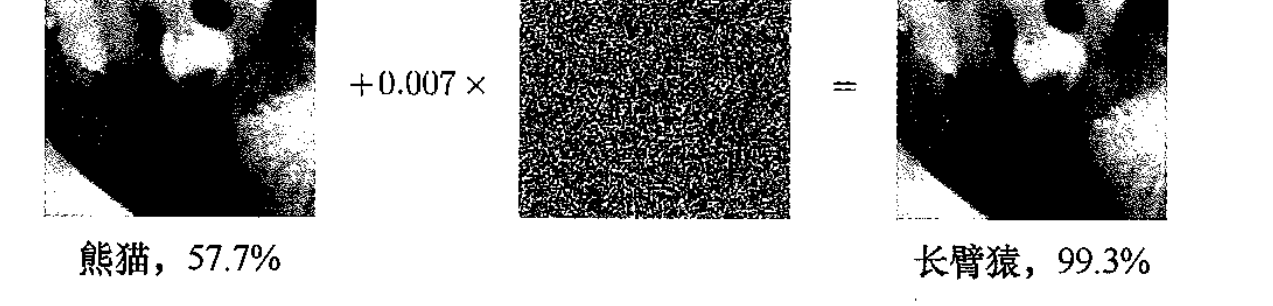
\includegraphics[width=0.72\textwidth]{ch10-fig10-16-对抗攻击.png}
  \caption{针对训练好的卷积网络的攻击示例。左边的图像以 $57.7\%$ 的置信度归类为熊猫。添加少量随机扰动（这些扰动本身以 $8.2\%$ 的概率归类为线虫），导致右边的图像以 $99.3\%$ 的置信度归类为长臂猿［经 Goodfellow, Shlens, and Szegedy (2014) 授权使用］。}
  \label{figure:ch10-对抗攻击}
\end{figure}

以这种方式欺骗神经网络会引发潜在的安全问题，因为它为攻击训练好的分类器创造了机会。这个问题似乎是由过拟合引起的，在过拟合中，具有较高拟合能力的模型已经精确地适应了特定的图像，使得输入中的微小变化会导致预测类概率的大幅变化。然而事实证明，一幅经过调整能使特定训练好的网络产生虚假输出的图像，在被输入其他网络时也会导致类似的虚假输出（Goodfellow, Shlens, and Szegedy, 2014）。此外，使用灵活性低得多的线性模型可以得到类似的对抗结果。人工对图像进行物理修改也可能导致这种现象。当把一幅规则的、未损坏的人工图像呈现给训练好的神经网络时，该网络也会给出错误的预测，如\cref{figure:ch10-物理停车标志}所示。虽然这些对抗攻击的基本类型可以通过对网络训练过程进行简单修改来解决，但更复杂的对抗攻击方法处理起来依然较为困难。了解这些结果的含义并缓解隐患仍然是一个开放的研究领域。

\begin{figure}[htbp]
  \centering
  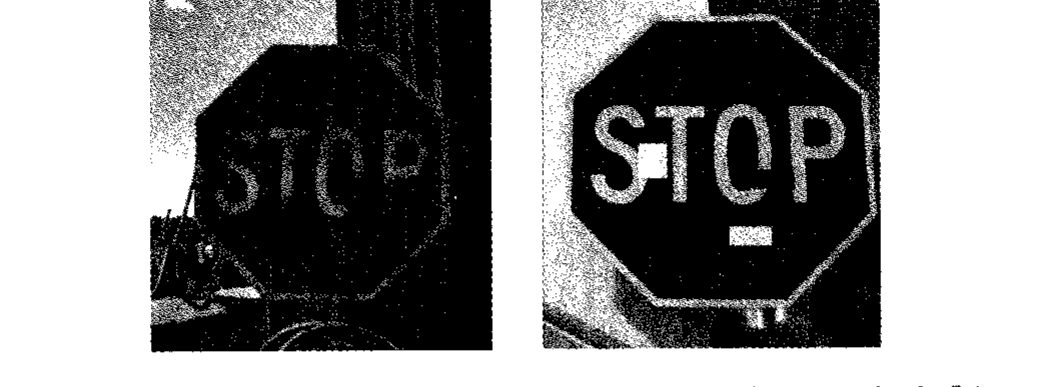
\includegraphics[width=0.6\textwidth]{ch10-fig10-17-停车标志.png}
  \caption{两个修改过的物理停车标志，它们会被 CNN 以极高的概率归类为限速标志［经 Eykholt et al. (2018) 授权使用］。}
  \label{figure:ch10-物理停车标志}
\end{figure}

\subsection{合成图像}\label{subsection:ch10-合成图像}

在关于图像修改的最后一个示例中，我们将讨论一种称为 DeepDream 的技术（Mordvintsev, Olah, and Tyka, 2015），它为运行训练好的卷积网络提供了额外的见解。它的目标是生成具有夸张特征的合成图像。为此，我们需要确定网络特定隐藏层中的哪些节点对特定图像有较强响应，然后修改图像从而放大这些响应。例如，我们将一些云的图像输入一个在对象检测任务上训练好的网络，并且如果一个特定节点在图像的特定区域检测到类似猫的模式，则将该区域修改得更像“猫”。

为此，我们首先将图像输入网络，并前向传播到某个特定层。然后将该层的反向传播 $\delta$ 变量设置为等于节点的预激活，并向输入层反向传播，从而获得图像像素的梯度向量（参见\cref{section:ch08-梯度计算}）。最后沿着梯度向量前进一小步来修改图像。该过程可以视作利用一种基于梯度的方法来增大函数的值（见\cref{exercise:ch10-10}）。要最大化的函数为
\begin{align}
  F(I)=\sum_{i,j,k}a_{ijk}(I)^2,
  \label{align:ch10-DeepDream目标}
\end{align}
其中 $a_{ijk}(I)$ 是当输入图像为 $I$ 时，所选网络层中通道 $k$ 的第 $i$ 行和第 $j$ 列单元的预激活，求和操作则涉及该层中所有的单元和通道。为了生成平滑的图像，可以使用空间平滑和像素裁剪形式的某些正则化。如果需要更强的增强效果，可以多次重复此过程。将 DeepDream 技术应用于图像的示例如\cref{figure:ch10-DeepDream}所示。有趣的是，即使卷积网络被训练以区分对象类别，但它们似乎至少能够捕获从这些类生成图像所需的一些信息。这种技术可以应用于照片，或者我们也可以将随机噪声作为输入，从而完全由训练好的网络生成图像。尽管 DeepDream 技术提供了一些关于训练好的网络运行的见解，但它主要用于生成艺术风格的有趣图像。

\begin{definition}[DeepDream]\label{definition:ch10-DeepDream}
设训练好的网络在输入 $I$ 上给出某层预激活 $a_{ijk}(I)$，$F$ 由\eqref{align:ch10-DeepDream目标}定义。从图像 $I_0$ 出发，按下式迭代
\begin{align}
  I_{\tau+1}=I_{\tau}+\eta\,\nabla_{I}F(I_{\tau}),\qquad \tau=0,1,2,\cdots,
  \label{align:ch10-DeepDream更新}
\end{align}
其中 $\eta>0$ 为步长，并对结果施加空间平滑与像素裁剪。称这一过程为 \textbf{DeepDream}。
\end{definition}

% SUPPLEMENT: parent=definition:ch10-DeepDream; kind=motivation; location=紧随其后的 remark（重构新增）
\begin{remark}（重构新增）
DeepDream 的定义把“让某个单元更兴奋”写成一个无约束的梯度上升问题，其目标函数\eqref{align:ch10-DeepDream目标}是所选层全部预激活的平方和，因此它不针对单一类别，而是放大该层已经学到的所有模式。平方的作用是让大幅激活主导目标（大响应的梯度也大），从而在合成图中产生夸张的纹理。定义中必须包含正则化：若不约束，梯度上升会把像素推到区间外并生成高频棋盘状结构，图像不再像自然图像；空间平滑与裁剪正是把迭代限制在“看起来像图像”的集合内。该过程不更新网络参数，只更新输入，这一点与训练有本质区别。
\end{remark}

\begin{proposition}[DeepDream 的上升方向]\label{proposition:ch10-DeepDream上升}
设 $F$ 在 $I$ 处可微，$\nabla_IF(I)\neq\mathbf{0}$。则对充分小的 $\eta>0$，沿\eqref{align:ch10-DeepDream更新}更新后目标函数严格增加：
\begin{align}
  F\bigl(I+\eta\nabla_IF(I)\bigr)>F(I).
  \label{align:ch10-DeepDream上升}
\end{align}
\end{proposition}
\begin{proof}
由可微性，$F(I+\eta\mathbf{g})=F(I)+\eta\,\mathbf{g}^{\mathsf{T}}\mathbf{g}+o(\eta\|\mathbf{g}\|)$，其中 $\mathbf{g}=\nabla_IF(I)$。于是
\begin{align*}
  \frac{F(I+\eta\mathbf{g})-F(I)}{\eta}=\|\mathbf{g}\|^2+\frac{o(\eta\|\mathbf{g}\|)}{\eta}\longrightarrow\|\mathbf{g}\|^2>0\qquad(\eta\to0^{+}).
\end{align*}
故存在 $\eta_0>0$，使 $0<\eta<\eta_0$ 时差商为正，即 $F(I+\eta\mathbf{g})>F(I)$。证毕。
\end{proof}

% SUPPLEMENT: parent=proposition:ch10-DeepDream上升; kind=motivation; location=紧随其后的 remark（重构新增）
\begin{remark}（重构新增）
这个命题说明 DeepDream 的每一步都在局部增加目标函数，前提是步长足够小且梯度非零。梯度为零时命题不适用：此时 $I$ 已是驻点，继续迭代不会带来一阶改进，实际算法会停止或需要更大的步长跳出。命题只保证“局部增加”，不保证 $F$ 有上界：\eqref{align:ch10-DeepDream目标}是预激活的平方和，若网络输出无界则 $F$ 无上界，迭代会不断放大像素，这正是需要正则化的数学理由。把该结论与\cref{proposition:ch10-快速梯度符号}对比可以看出两者是同一事实的两面：一个沿梯度上升以最大化目标，一个沿符号梯度上升以在无穷范数预算内最大化误差。
\end{remark}

\begin{figure}[htbp]
  \centering
  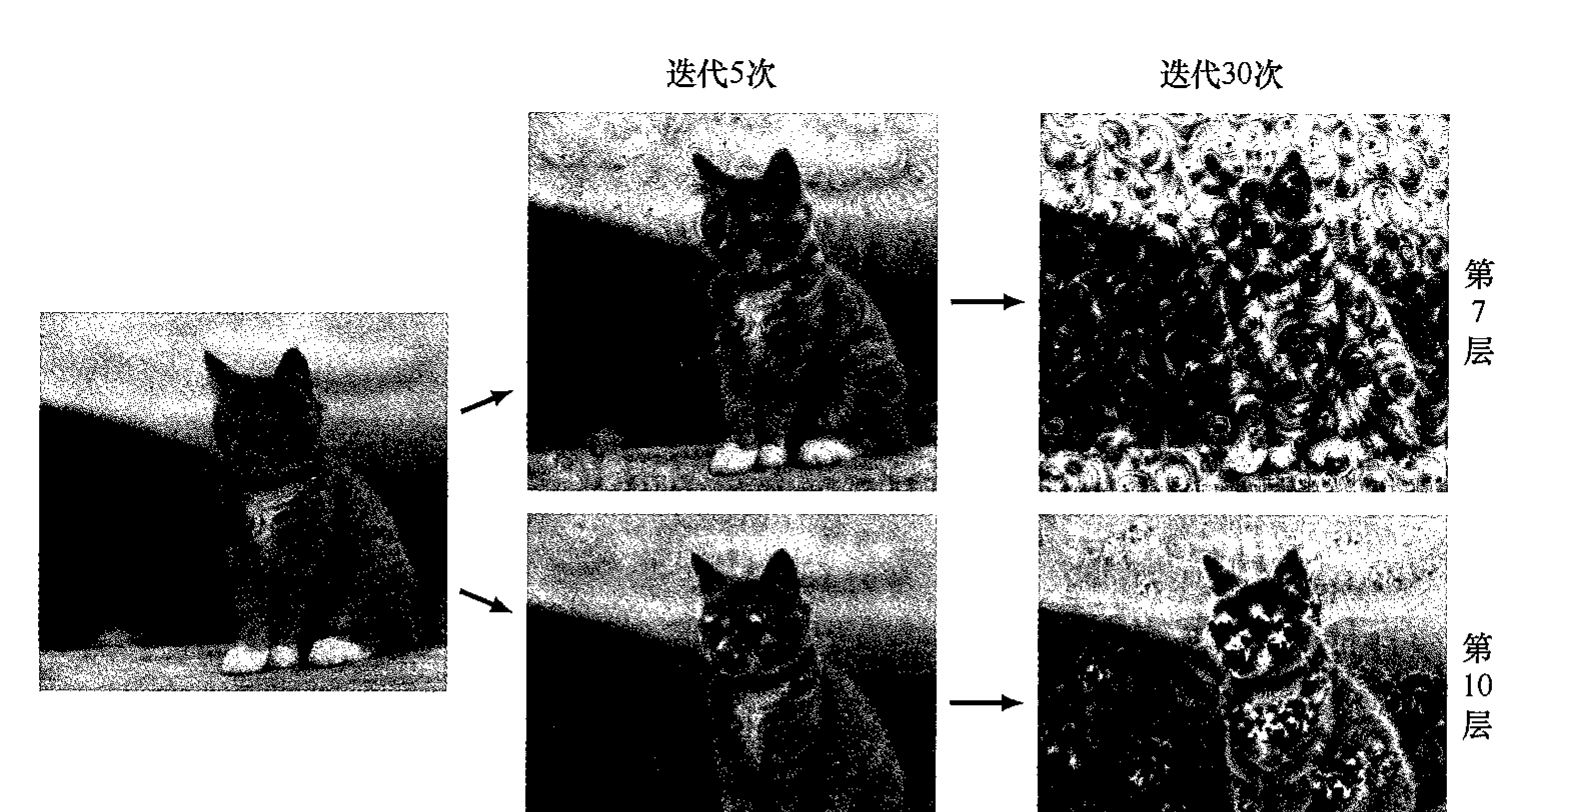
\includegraphics[width=0.92\textwidth]{ch10-fig10-18-deepdream.png}
  \caption{将 DeepDream 技术应用于图像的示例。上方显示了在经过 5 次迭代和 30 次迭代后，应用算法到 VGG-16 模型的第 7 个卷积层激活的结果。类似地，下方显示了同样在经过 5 次迭代和 30 次迭代后，应用算法到 VGG-16 模型的第 10 个卷积层激活的结果。}
  \label{figure:ch10-DeepDream}
\end{figure}

\end{document}
